\documentclass[11pt]{article}
\usepackage[margin=0.75in]{geometry}
\usepackage{tikz}
\usepackage{amsmath}
\usepackage{amssymb}
% \usepackage{xcolor}
\usepackage{enumitem}
\usetikzlibrary{arrows.meta, patterns, positioning}

\usepackage[dvipsnames]{xcolor}

% Custom colors
\definecolor{carrierred}{RGB}{200,30,30}
\definecolor{sbplus}{RGB}{220,120,0}
\definecolor{sbminus}{RGB}{210,80,150}

\begin{document}

\begin{center}
    \textbf{In-class Tutorial: Coupled Cavities (Part 2)}\\
    March 25, 2026\\
    Lasers and Optomechanics\\~\\
    Name: \underline{\hspace{10cm}}
\end{center}


\noindent
\textbf{Coupled Cavity Sensing Matrix}\\
In Part 1, we learned about a coupled cavity and compound interferometers, and explored the basics of the coupled cavity resonance.
In Part 2, we will learn how to sense the PDH signals for the two degrees of freedom $L_1$ and $L_2$. 
This will form our \textit{sensing matrix}, which can be used to simultaneously detect and feed back to the mirror locations to keep our interferometer on the desired resonant points (derived in Part 1 to be $\phi_{1,0} = \phi_{2,0} = 0$ for carrier and $\phi_{1,\Omega} = \phi_{2,\Omega} = \dfrac{\pi}{2}$ for the RF sidebands.)


\begin{center}
  
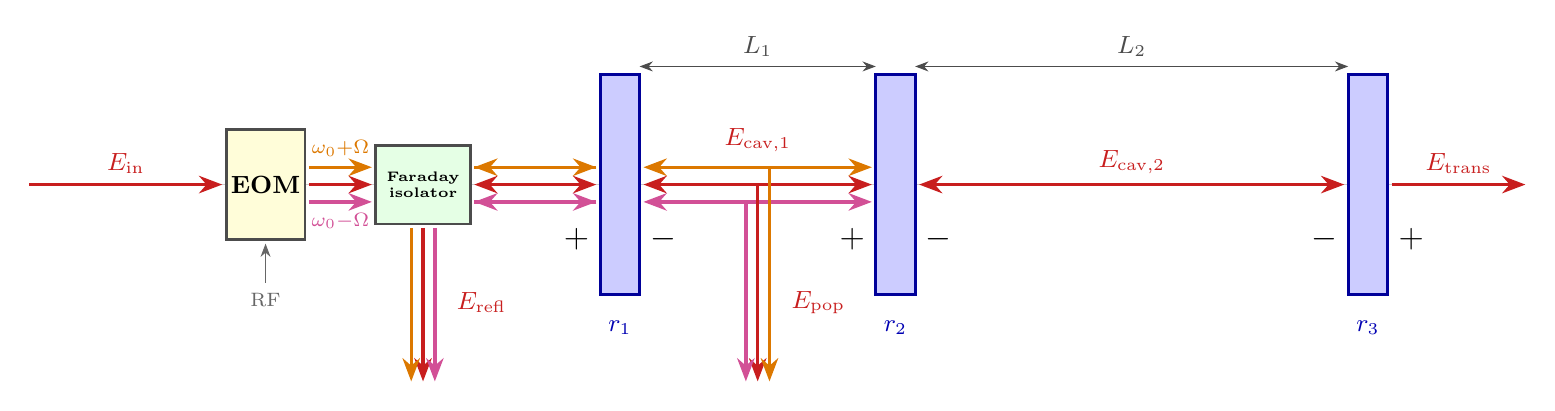
\begin{tikzpicture}[
    >=Stealth,
    thick,
    carrier/.style={->, very thick, carrierred},
    sbp/.style={->, very thick, sbplus},
    sbm/.style={->, very thick, sbminus},
]

%--- Coordinates ---
\def\rIx{0}         % r1 center x (input coupler)
\def\rIIx{3.5}      % r2 center x (coupling mirror)
\def\rIIIx{9.5}     % r3 center x (end mirror)
\def\mirH{1.4}      % half-height of mirrors
\def\mirW{0.25}     % half-width of mirror rectangles
% EOM box
\def\EOMx{-4.5}     % EOM center x
\def\EOMw{0.5}      % EOM half-width
\def\EOMh{0.7}      % EOM half-height
% Faraday isolator
\def\FIx{-2.5}      % FI center x
\def\FIy{0}
\def\FIw{0.6}       % FI half-width
\def\FIh{0.5}       % FI half-height
% Reflected beam drop
\def\Yrefl{-2.5}    % y level for downward E_refl exit

%--- Cavity axis (thin guide line) ---
\draw[gray!40, thin] (-7.5, 0) -- (\rIIIx+2.0, 0);

%============================================================
% EOM
%============================================================
\filldraw[fill=yellow!15!white, draw=black!70, line width=1pt]
    (\EOMx-\EOMw, -\EOMh) rectangle (\EOMx+\EOMw, \EOMh);
\node[font=\small\bfseries] at (\EOMx, 0) {EOM};
\draw[->, thin, black!60] (\EOMx, -\EOMh-0.55) -- (\EOMx, -\EOMh-0.05)
    node[below, font=\scriptsize, pos=0] {RF};

%============================================================
% Faraday isolator
%============================================================
\filldraw[fill=green!10!white, draw=black!70, line width=1pt]
    (\FIx-\FIw, \FIy-\FIh) rectangle (\FIx+\FIw, \FIy+\FIh);
\node[font=\tiny\bfseries, align=center] at (\FIx, \FIy) {Faraday\\isolator};

%============================================================
% Input beam: single carrier, left to EOM
%============================================================
\draw[carrier] (-7.5, 0) -- (\EOMx-\EOMw-0.05, 0)
    node[midway, above, font=\small] {$E_\mathrm{in}$};

%============================================================
% EOM to Faraday isolator: carrier + sidebands
%============================================================
\draw[carrier] (\EOMx+\EOMw+0.05, 0) -- (\FIx-\FIw-0.05, 0);
\draw[sbp] (\EOMx+\EOMw+0.05,  0.22) -- (\FIx-\FIw-0.05,  0.22)
    node[midway, above, font=\scriptsize] {$\omega_0{+}\Omega$};
\draw[sbm] (\EOMx+\EOMw+0.05, -0.22) -- (\FIx-\FIw-0.05, -0.22)
    node[midway, below, font=\scriptsize] {$\omega_0{-}\Omega$};

%============================================================
% Faraday isolator to r1: double-headed carrier + sidebands
%============================================================
\draw[carrier, {Stealth}-{Stealth}] (\FIx+\FIw+0.05, 0) -- (\rIx-\mirW-0.05, 0);
\draw[sbp] (\FIx+\FIw+0.05,  0.22) -- (\rIx-\mirW-0.05,  0.22);
\draw[sbm] (\FIx+\FIw+0.05, -0.22) -- (\rIx-\mirW-0.05, -0.22);

%============================================================
% r1 -- input coupler
%============================================================
\filldraw[fill=blue!20!white, draw=blue!60!black, line width=1.2pt]
    (\rIx-\mirW, -\mirH) rectangle (\rIx+\mirW, \mirH);
\node[below, blue!70!black, font=\small] at (\rIx, -\mirH-0.2) {$r_1$};
\node[font=\large, black] at (\rIx-\mirW-0.3, -0.7) {$+$};
\node[font=\large, black] at (\rIx+\mirW+0.3, -0.7) {$-$};

%============================================================
% Cavity 1 (r1 to r2): carrier + sidebands all resonate here
%============================================================
\draw[carrier, {Stealth}-{Stealth}] (\rIx+\mirW+0.05, 0) -- (\rIIx-\mirW-0.05, 0)
    node[midway, above=8pt, font=\small] {$E_\mathrm{cav,1}$};
\draw[sbp, {Stealth}-{Stealth}] (\rIx+\mirW+0.05,  0.22) -- (\rIIx-\mirW-0.05,  0.22);
\draw[sbm, {Stealth}-{Stealth}] (\rIx+\mirW+0.05, -0.22) -- (\rIIx-\mirW-0.05, -0.22);

%============================================================
% r2 -- coupling mirror (HR sides face both cavities)
%============================================================
\filldraw[fill=blue!20!white, draw=blue!60!black, line width=1.2pt]
    (\rIIx-\mirW, -\mirH) rectangle (\rIIx+\mirW, \mirH);
\node[below, blue!70!black, font=\small] at (\rIIx, -\mirH-0.2) {$r_2$};
\node[font=\large, black] at (\rIIx-\mirW-0.3, -0.7) {$+$};
\node[font=\large, black] at (\rIIx+\mirW+0.3, -0.7) {$-$};

%============================================================
% Cavity 2 (r2 to r3): carrier only, sidebands do not enter
%============================================================
\draw[carrier, {Stealth}-{Stealth}] (\rIIx+\mirW+0.05, 0) -- (\rIIIx-\mirW-0.05, 0)
    node[midway, above, font=\small] {$E_\mathrm{cav,2}$};

%============================================================
% r3 -- end mirror
%============================================================
\filldraw[fill=blue!20!white, draw=blue!60!black, line width=1.2pt]
    (\rIIIx-\mirW, -\mirH) rectangle (\rIIIx+\mirW, \mirH);
\node[below, blue!70!black, font=\small] at (\rIIIx, -\mirH-0.2) {$r_3$};
\node[font=\large, black] at (\rIIIx-\mirW-0.3, -0.7) {$-$};
\node[font=\large, black] at (\rIIIx+\mirW+0.3, -0.7) {$+$};

%============================================================
% Transmitted beam: carrier only exiting right of r3
%============================================================
\draw[carrier] (\rIIIx+\mirW+0.05, 0) -- (\rIIIx+2.0, 0)
    node[midway, above, font=\small] {$E_\mathrm{trans}$};

%============================================================
% Reflected beams: sidebands from r1 back to FI, then drop down
%============================================================
\draw[sbp] (\rIx-\mirW-0.05,  0.22) -- (\FIx+\FIw+0.05,  0.22);
\draw[sbm] (\rIx-\mirW-0.05, -0.22) -- (\FIx+\FIw+0.05, -0.22);

% Downward exits from bottom of Faraday isolator
\draw[carrier] (\FIx,      -\FIh-0.05) -- (\FIx,      \Yrefl);
\draw[sbp]     (\FIx-0.15, -\FIh-0.05) -- (\FIx-0.15, \Yrefl);
\draw[sbm]     (\FIx+0.15, -\FIh-0.05) -- (\FIx+0.15, \Yrefl);
\node[right, font=\small, carrierred] at (\FIx+0.15+0.15, {0.5*(-\FIh+\Yrefl)}) {$E_\mathrm{refl}$};
% \draw[carrier] (\FIx+0.15+0.15) -- (0.5*(-\FIh+\Yrefl))
%     node[right, font=\small] {$E_\mathrm{refl}$};

%============================================================
% POP beams: sidebands from r1 back to FI, then drop down
%============================================================

% Downward exits from bottom of Faraday isolator
\draw[carrier] (0.5*\rIx+0.5*\rIIx,      0) -- (0.5*\rIx+0.5*\rIIx,      \Yrefl);
\draw[sbp]     (0.5*\rIx+0.5*\rIIx+0.15, +0.22) -- (0.5*\rIx+0.5*\rIIx+0.15, \Yrefl);
\draw[sbm]     (0.5*\rIx+0.5*\rIIx-0.15, -0.22) -- (0.5*\rIx+0.5*\rIIx-0.15, \Yrefl);
\node[right, font=\small, carrierred] at (0.5*\rIx+0.5*\rIIx+0.15+0.15, {0.5*(-\FIh+\Yrefl)}) {$E_\mathrm{pop}$};

%============================================================
% Dimension annotations
%============================================================
% L1: r1 right face to r2 left face
\draw[<->, thin, black!70]
    (\rIx+\mirW, \mirH+0.1) -- (\rIIx-\mirW, \mirH+0.1)
    node[midway, above, font=\small] {$L_1$};
% \draw[dotted, thin, gray] (\rIx+\mirW,  -\mirH-0.25) -- (\rIx+\mirW,  -\mirH-1.0);
% \draw[dotted, thin, gray] (\rIIx-\mirW, -\mirH-0.25) -- (\rIIx-\mirW, -\mirH-1.0);

% L2: r2 right face to r3 left face
\draw[<->, thin, black!70]
    (\rIIx+\mirW, \mirH+0.1) -- (\rIIIx-\mirW, \mirH+0.1)
    node[midway, above, font=\small] {$L_2$};
% \draw[dotted, thin, gray] (\rIIx+\mirW,  -\mirH-0.25) -- (\rIIx+\mirW,  -\mirH-1.0);
% \draw[dotted, thin, gray] (\rIIIx-\mirW, -\mirH-0.25) -- (\rIIIx-\mirW, -\mirH-1.0);

\end{tikzpicture}


\end{center}

\noindent \textbf{Figure 1:} Coupled-cavity interferometer, with three mirrors aligned and carrier (red) plus one set of RF sidebands (pink and orange) incident.  
Also labeled is the REFL and POP fields, standing for the reflection and pick-off ports.

Recall the coupled cavity equations from Part 1's solutions are 
\begin{align}
\label{eq:cc_refl}
r(\phi_1,\phi_2) = \dfrac{E_\mathrm{refl}}{E_\mathrm{in}}(\phi_1,\phi_2) &= \dfrac{r_1 - r_1 r_2 r_3 e^{- i 2 \phi_2} + r_2 e^{-i 2 \phi_1} - r_3 e^{-i 2 (\phi_1 + \phi_2)}}{1 + r_1 r_2 e^{-i 2 \phi_1} - r_2 r_3 e^{-i 2 \phi_2} - r_1 r_3 e^{-i 2 (\phi_1 + \phi_2)}}\\
\label{eq:cc_cav1}
g_1(\phi_1,\phi_2) = \dfrac{E_\mathrm{cav,1}}{E_\mathrm{in}}(\phi_1,\phi_2) &= \dfrac{t_1 (1 - r_2 r_3 e^{-i 2 \phi_2}) }{1 + r_1 r_2 e^{-i 2 \phi_1} - r_2 r_3 e^{-i 2 \phi_2} - r_1 r_3 e^{-i 2 (\phi_1 + \phi_2)}}\\
\label{eq:cc_cav2}
g_2(\phi_1,\phi_2) = \dfrac{E_\mathrm{cav,2}}{E_\mathrm{in}}(\phi_1,\phi_2) &= \dfrac{t_1 t_2 e^{-i \phi_1}}{1 + r_1 r_2 e^{-i 2 \phi_1} - r_2 r_3 e^{-i 2 \phi_2} - r_1 r_3 e^{-i 2 (\phi_1 + \phi_2)}}\\
\label{eq:cc_trans}
t(\phi_1,\phi_2) = \dfrac{E_\mathrm{trans}}{E_\mathrm{in}}(\phi_1,\phi_2) &= \dfrac{t_1 t_2 t_3 e^{-i (\phi_1 + \phi_2)}}{1 + r_1 r_2 e^{-i 2 \phi_1} - r_2 r_3 e^{-i 2 \phi_2} - r_1 r_3 e^{-i 2 (\phi_1 + \phi_2)}}
\end{align} 
where $r_i, t_i$ the $i$th mirror reflectivity and transmissions.

Also recall the simplified PDH error signal expression for a Fabry-Perot (See PDH tutorial and solutions):
\begin{align}
    \label{eq:pdh_error}
    P_\mathrm{PDH} = i \dfrac{\Gamma}{2} P_\mathrm{in} \left(f(\phi_0)^* f(\phi_0 - \phi_{rf}) - f(\phi_0) f(\phi_0 + \phi_{rf})^* \right)
\end{align}
where $f$ represents the Fabry-Perot field transfer function from input to any port.

\newpage 
\noindent
\textbf{Coupled Cavity Degrees of Freedom}

When dealing with complex interferometers with multiple fields resonating inside of them, 
it can be difficult to parse exactly what signals our photodetectors are sensing,
and how they are related to the motion of different optics.
For instance, consider what happens if the middle mirror of our coupled cavity moves.
All three of our fields will respond to that motion, the carrier $\omega_0$ and RF sidebands $\omega_0 \pm \Omega$.

For simplicity, let's consider the end mirror $r_3$ motion about it's nominal resonance point, $\phi_1 = \phi_2 = 0$.    
End mirror motion will \textit{only} move $L_2$, and will modulate \textit{only} the carrier~\textcolor{Mahogany}{\footnote{\textcolor{Mahogany}{The above statement ``End mirror motion will modulate only the carrier'' is not strictly true, as some sideband light always enters the arm cavity.  The RF sideband light is simply antiresonant in the arm cavity, so the response is greatly reduced compared to carrier.}}}.
Let's call this end mirror motion about nominal $\Delta \phi_2$.

Equation~\ref{eq:pdh_error} gives us a general complex expression for calculating the PDH error signal at any port of a Fabry-Perot interferometer.  
One can imagine replacing the Fabry-Perot transfer functions $f(\phi)$ with the coupled cavity transfer functions $c(\phi_1,\phi_2)$ from Eqs~\ref{eq:cc_refl}-\ref{eq:cc_trans}.
Then, we could imagine using that coupled-cavity PDH error function to calculate the PDH discriminate about $\phi_2 = 0$: $\Delta P_\mathrm{PDH} / \Delta \phi_2$. 

\noindent~\\
\textbf{Sensing Matrix}

A \textit{sensing matrix} takes an interferometer degree of freedom's motion in radians about it's nominal position, 
like $\Delta \phi_1$ and $\Delta \phi_2$, 
and converts it to detected photodetector signal in watts.
The photodetector signal can in general be DC light or RF-demodulated PDH IQ signals.
In this example, we'll focus on constructing the following sensing matrix:

\begin{align}
\begin{bmatrix}
    P_\mathrm{refl}^I \\[2ex]
    P_\mathrm{refl}^Q \\[2ex]
    P_\mathrm{pop}^I \\[2ex]
    P_\mathrm{pop}^Q
\end{bmatrix} = \begin{bmatrix}
    \dfrac{\Delta P_\mathrm{refl}^I}{\Delta \phi_1} & \dfrac{\Delta P_\mathrm{refl}^I}{\Delta \phi_2} \\[2ex]
    \dfrac{\Delta P_\mathrm{refl}^Q}{\Delta \phi_1} & \dfrac{\Delta P_\mathrm{refl}^Q}{\Delta \phi_2} \\[2ex]
    \dfrac{\Delta P_\mathrm{pop}^I}{\Delta \phi_1} & \dfrac{\Delta P_\mathrm{pop}^I}{\Delta \phi_2} \\[2ex]
    \dfrac{\Delta P_\mathrm{pop}^Q}{\Delta \phi_1} & \dfrac{\Delta P_\mathrm{pop}^Q}{\Delta \phi_2}
\end{bmatrix}
\begin{bmatrix}
    \Delta \phi_1 \\[2ex]
    \Delta \phi_2
\end{bmatrix}
\end{align}

The sensing matrix converts interferometer motion in radians 
to real power signals on our diodes in watts: each matrix element is the \textit{PDH discriminant} in $\mathrm{W/rad}$.
Both $\Delta \phi_1$ and $\Delta \phi_2$ will contribute to a signal appearing in any diode, but the sensing matrix element sizes can help us decipher where signals appear strongest.

In the end, the sensing matrix is extremely useful because once it is calculated, 
it can be \textit{inverted} to be used in control systems.
The inverted sensing matrix directs photodetector signals to specific degrees of freedom, then to actuators meant to control those degrees of freedom.
Inverting sensing matrices is sometimes extremely difficult if two degrees of freedom are largely degenerate.
This is the game LIGO commissioners play fairly regularly at the site~\textcolor{Plum}{\footnote{\textcolor{Plum}{In the game of interferometry, you lock or you die}}}.


\noindent~\\
\textbf{Assembly of a Coupled Cavity Sensing Matrix}

\textbf{1. Construct and evaluate a sensing matrix for the CARM coupled cavity of Advanced LIGO.} 
It is typical for $\phi_1$ and $\phi_2$ to be separated into two degrees of freedom called PRCL and CARM, respectively~\textcolor{OliveGreen}{\footnote{\textcolor{OliveGreen}{Of course, Advanced LIGO has two arms, but they both can be combined together into one arm through the compound interferometer technique perfomed on the Michelson.}}}.  
The detection ports should be the REFL and POP I and Q quadratures.
Assume a lossless interferometer with $T_1 = 3.1\%$, $T_2 = 1.5\%$, $T_3 = 5~\mathrm{ppm}$, $L_1 = 56~\mathrm{m}$, and $L_2 = 4000~\mathrm{m}$.
You will need an algebra helper or python script to calculate this.






\end{document}